\subsection{August 17, 2008}
\subsubsection*{The Background}
Last night, I drew another card to ponder for the next day or so and
picked the Nine of Swords from the Universal Waite deck\cite{tarotRWS}.
This card contains a distressing image of someone buried deep in
emotional agony, sitting up in bed while nine swords hang in the air
above and behind them.  While the card usually stands for that
withdrawal into self that comes with tsuch emotional pain, it can also
represent, particularly while reversed or ill-dignified, oppression.  In
fact, Rachel Pollack specifically mentions sexuality as the reason for
the oppression, and that brought to mind work.

At my day job, working as technical support in the campus library, my
direct supervisor quit late last year and was replaced with someone
twice as competent as he was.  My old supervisor was very good at
keeping the library up and running, and my new supervisor is better,
going further by doing things to make the library work even more
smoothly.  However, while my old supervisor acted fairly immature and
made crude jokes ceaselessly, my new supervisor far outstrips him in
this category, with every word and action showing the twelve-year-old
that he still thinks he is.

While I don't believe that he is actively oppressing me because of my
sexuality --- I doubt he even knows, and they are pretty clearly jokes,
my Indonesian coworker gets his fair share of terrorist jokes --- it
does lead to a decidedly uncomfortable environment to be working in at
times.  Perhaps I'm just a sensitive person, but I would enjoy not
having this stigma hanging over my workplace.  How can I work more
effectively with this?  Is coming out to my boss the right thing, or
should I follow my own suggestion and not let my sexuality interfere
with my job, since the former has no place in the latter?

\subsubsection*{The Drawing}
Still using the Universal Waite deck, I decided to make up a spread on
the spot.  The layout would consist of two piles related to two `header'
cards.  One header card would stand for what I saw in my boss and the
other would stand for a different view-point on the situation: that of 
my boss.  I would draw two cards at a time, one for each pile,
and read the two cards in a general matter to gain perspective on the
situation, drawing until I feel that I've got a better idea of what's
going on.

\begin{itemize}
  \item Theme for the reading: Nine of Swords
  \item My header card: Knight of Cups.
  \begin{enumerate}
    \item Four of Pentacles
    \item Five of Wands
    \item The Devil
    \item Six of Wands
  \end{enumerate}
  \item The other header card: Knight of Wands.
  \begin{enumerate}
    \item King of Wands
    \item Four of Swords
    \item Death
    \item Eight of Swords
  \end{enumerate}
  \item Final card: Ace of Wands
\end{itemize}
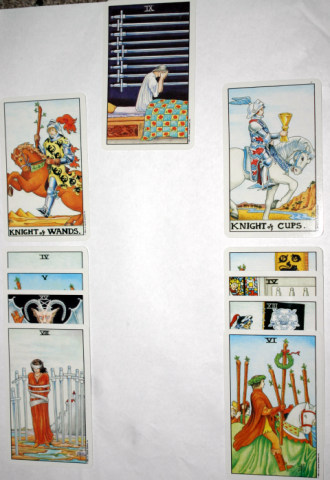
\includegraphics{image8-17-08.png}

\subsection*{The Reading}
I initially selected the header card for my boss, since his attitude at
work recently has reminded me of little else, what with the way the
Knight of Wands rushes into battle, usually without any sort of plan.
Recently, my boss has been fixing things `shotgun style' at work, just
replacing parts and hoping they're the right ones, and that replacing
them will fix the issue.  I chose my own header card in much the same
way, with the Knight of Cups' more reticent nature, particularly as
applied to how I feel about dealing with my boss.  It wasn't until I got
halfway through the spread that I noticed that they were elementally
ill-disposed towards one another.

Looking at my boss's header card, the first thing I notice in the picture
itself is the flashiness of the uniform.  My boss doesn't dress flashy,
but he does act in such a way as to draw attention to himself, and I
find this particularly apt.  In my own card, I first noticed that the
Knight doesn't look at anything other than the cup, keeping his fist
wrapped tightly around his horse's reigns, even though it looks as if
the horse would really rather like a drink of that stream in front of
him.  For myself, I see this as me focusing a little too hard on this
issue, perhaps at the expense of those issues around me.  The rest of
the reading proceeded more as a dialog.

I drew the first two cards at once and laid them beneath the two header
cards: the Four of Pentacles and the King of Wands.  The traditional
meaning of the King was not, as I found, very applicable.  Instead, the
card, as being a vertical transmutation of my boss's Knight, very
plainly spoke of my desires for my boss to grow up.  His homophobic
jokes are so\ldots high-school.  Not only am I in college, but he is
nearing thirty, and it's well past time for him to get on with work and
out of this party stage.  His card, on the other hand, spoke of
defenses.  The miser in the Four of Pentacles protects his heart and
mind with defensive layers, and even his feet are covered to, perhaps
inadvertently, block that symbolic connection with the earth and thus
everyone else.  This card responded to the King by saying, ``I use that
humor to cover up and hide problems deeper than this.''

The second two cards were drawn.  My Four of Swords suggests relaxation,
retreating from the while, taking things in stock.  I believe that this
is me telling my boss to relax, calm down, maybe step back and take in
the world from a different point of view rather than rushing forward.
Perhaps then he would be easier to reason with, rather than attempting
to talk with that joker of a mask he wears.  In response, his Five of
Wands suggested that there is no real reason to do such a thing.  ``Life
is just a game,'' it said.  ``So long as we follow the rules and do our
jobs, it doesn't matter.''

My exasperation was brought forth in the the next two cards, both Major
Arcana.  Death, for my card, begged for change and transition.  ``The
game needs to change --- you need to change --- so that we can both do
our jobs more effectively''  My boss's card, the Devil, shrugs that off
with comfort and complacency.  ``This may not be my true self, and may
just be a mask, but there's no reason to change; you know and I know
that neither of us are too enthused about our jobs and they're hardly
challenging either of us.  Office humor helps keep things sane for both
of us, and you know that.''

At this point in the reading, I felt like I had a better grasp on the
situation.  I know my boss really is just joking: whether he is
homophobic or not doesn't enter into it much at all, I think --- this is
just a way to keep himself sane at work.  However, it is affecting the
way I feel about my job and the way I perform at work, to a small
extent.  Rather than joining in conversations at work as I used to, I'm
more inclined to just sit and listen, unwilling to participate in the
things I disagree with.  

The social activist Unitarian in me would like
to tell my boss how inappropriate that is in any setting; while I'm
hardly `tough', there are those that aren't as thick-skinned as I am
when it comes to this sort of thing, and he should avoid being hurtful
towards anyone.  Still, I'm wary of opening up in this situation lest it
make things strained between my boss and myself, or, worse, that he'll
get in trouble with someone higher up than him --- as I mentioned
before, he really turned the workplace around, productivity-wise.
Curious and willing to try, I drew two more cards with the intent of
seeing how this dynamic may extend into the future.

The Eight of Swords shows a woman actively oppressed, bound and
blindfolded and surrounded by swords.  However, her oppressors are
nowhere in sight and the swords only block her on one side.  This is an
oppression that she has come to expect, whether out of cynicism or
weakness.  If I were to accept my oppression like this card suggests
being under my heading, then my boss's card, the Six of Swords, may be
in his future: Victory.  The man rides crowned on his horse, riding in a
victory parade, completely unharmed.  He has done nothing and he has
won and I have lost, dignity trampled.

Frustrated, I drew one final card, just to look for something more
optimistic.  The Ace of Wands is just what I needed.  The embodiment of
the energy of the Wands, happiness and joy as a gift from that inner
strength I know we all have.  I know what I have to do.

I will have to confront my boss on this matter soon.
